\chapter{Marco Teórico}
\label{chap:marcoteorico}
%\endinput
% Estado del arte general de la temática de estudio. 
\section{Introducci\'on}

Para el an\'alisis de posibles colisiones es necesario evaluar de forma anticipada las trayectorias de todos los objetos que orbitan la Tierra y detectar los acercamientos de riesgo. Si la predicci\'on de las posiciones fuera exacta, este estudio s\'olo implicar\'ia un esfuerzo computacional a resolver. No obstante, el movimiento orbital de los objetos no es ideal y las posiciones medidas o estimadas siempre acarrean una indeterminaci\'on, y m\'as a\'un cuando se trata de desechos.\\

La t\'ecnica de detecci\'on de encuentros, consiste en realizar propagaciones de las posiciones de todo el cat\'alogo una semana hacia el futuro, definir un volumen seguro rodeando al sat\'elite de inter\'es, y si alg\'un objeto externo se introduce dentro del volumen de riesgo, es decir, se acerca a una distancia m\'inima por debajo del umbral determinado, se considera una situaci\'on de riesgo.\\ Esta metodolog\'ia no tiene en cuenta los errores en la determinaci\'on de la posici\'on de los objetos, y por lo general deriva en falsas alarmas, con las que se corre el riesgo de realizar maniobras innecesarias.\\
Una vez identificado un encuentro, para un estudio m\'as exhaustivo de la situaci\'on, adem\'as de la m\'inima distancia de acercamiento o {\it{miss distance}}, se calcula la {\bf{probabilidad de colisi\'on}}: PoC.  Esta \'ultima ofrece un panorama m\'as completo ya que incorpora los errores en las posiciones a trav\'es de las matrices de covarianza.\\

Como ya mencionamos (Sec. \ref{subsec:estudiocolision}), en este trabajo nos enfocamos en analizar las situaci\'ones de encuentro ya identificadas y en particular, aquellas que involucran a misiones operativas y desechos espaciales.\\

La posici\'on de la misi\'on operativa y los errores asociados a la misma, la provee el departamento de din\'amica orbital (Sec. \ref{sec:posMision}).
La posici\'on de los desechos, s\'olo es posible conocerla, utilizamos los datos p\'ublicos que ofrece el comando de defensa norteamericano, \ac{NORAD} a trav\'es de su p\'agina Space-Track {\footnote{http://www.space-track.org}}. Las posiciones son publicadas en formato \ac{TLE} (Sec. \ref{subsec:tleformat}), sin errores asociados, y son propagadas hasta el momento del encuentro con el modelo SGP4  \citep{hoots1980spacetrack}, que tampoco ofrece informaci\'on sobre los errores de propagaci\'on.\\

En este cap\'itulo, en primer lugar presentamos la forma en que se comunican los acercamientos de riesgo (Sec. \ref{sec:anuncio}), por ejemplo mediante \ac{CDM}. Luego describimos las distintas determinaciones en las posiciones y los formatos en que se presentan. En el caso del formato TLE, dedicamos un \'item para presentar el modelo de propagaci\'on SGP4 (Sec. \ref{sec:sgp4model})\\
Para el estudio de la estimaci\'on de errores, detallamos el m\'etodo de Osweiler \citep{Osweiler} que permite la construcci\'on de las matrices de covarianza a partir de un conjunto de TLEs, cuando no se cuenta con datos m\'as precisos.\\
Una vez calculada la matriz de covarianza con el m\'etodo de Osweiler, ser\'a necesario propagarla al instante predicho para el encuentro. Para ello proponemos la implementaci\'on de una tabla con valores estad\'isticos inferidos del an\'alisis de datos de la misi\'on.\\
Finalmente detallamos el algoritmo para el c\'alculo de la PoC.\\

\section{Comunicaciones de riesgos de colisi\'on}{\label{sec:anuncio}}
\textcolor{red}{considerar: time code formats, y xml, ccsds 301.0-b-4 y ccsds 505.0-b-1}

Desde el momento en que la superpoblaci\'on del espacio empez\'o a analizarse desde un punto de vista de riesgo, las agencias u organismos capaces de rastrear el ambiente espacial, fueron las primeras en implementar sistemas de comunicaci\'on para advertir sobre posibles colisiones. (\textcolor{red}{se puede ampliar en contexto historico, mencionando a NASA y al CSM})\\
El sistema de alertas fue evolucionando a medida que los controles del \'ambito espacial fueron increment\'andose y tomando caracter internacional. Las comunicaciones que en sus or\'igenes eran mails particulares, fueron tomando un car\'acter formal y estandarizado, hasta que finalmente en Junio del 2013 el consejo consultivo para los sistemas de datos espaciales, \ac{CCSDS}, public\'o el mensaje est\'andard recomendado, el: \ac{CDM} \citep{CDMstd}.\\

\subsection{El CDM}

Es un mensaje estandarizado para el intercambio de informaci\'on entre los organismos capaces de detectar acercamientos y los due\~nos y operadores de los objetos involucrados en el encuentro.\\
Los CDM se env\'ian a los operadores a cargo y/o se disponibilizan en la p\'agina de space-track para usuarios con permisos especiales 72 hs antes del encuentro.
Su formato estandarizado unifica la informaci\'on que all\'i se publica y facilita la interoperatibilidad sin ambig\"{u}edades. As\'i mismo, permite la automatizaci\'on de procesos de detecci\'on y an\'alisis de las situaciones de riesgo y ofrece la informaci\'on con tiempo suficiente para la toma de decisiones.\\

Los CDMs contienen datos del encuentro como: la m\'inima distancia, la probabilidad de colisi\'on, el tiempo del m\'aximo aceramiento y los vectores de posici\'on y velocidad relativa en el momento del m\'aximo aceramiento.
Para la generaci\'on de los mismos se consideran criterios de emergencia, seg\'un ocurra que el acercamiento entre los objetos es:\\

LEO:\\
overall miss distance < 1km\\
radial miss distance < 200m\\
GEO/MEO:\\
Overall miss distance < 10 km.\\

Son mensajes exclusivamente informativos, que no imprimen recomendaciones ni sugerencias de acci\'on.
Y es importante destacar que muchas veces para las estimaciones, los centros de c\'omputo no cuentan con maniobras planificadas en sus predicciones.\\ 

El mismo se distribuye en distintos formatos ...ampliar ...CCSDS standard para el CDM. \\
\textcolor{red}{Incorporar formato}

{\bf{FORMAT (poner un ejemplo)}}\\
El CDM es un mensaje codificado en formato ASCII, que puede distribuirse mediante un texto plano (KVN), o por medio de un XML. 
En el sistema planteado es recomendable que en el documento de interfaces, se especifique con qu\'e formato se va a realizar el intercambio.\\
{\bf{Notaci\'on de Unidades}}\\
El CDM utiliza unidades del \ac{SI} con la siguiente nomenclatura:\\
\begin{itemize}
 \item km: kil\'ometros.
 \item m: metros.
 \item d: d\'as, 86400 segundos del SI.
 \item s: segundos.
 \item kg: kilogramos.
 \item W: watts.
 \item \%: porcentaje.
\end{itemize}

El CDM contiene informaci\'on de un \'unico encuentro, entre dos objetos, OBJ1 y OBJ2.\\
Ofrece:\\
\begin{itemize}
 \item Las posiciones de OBJ1 y OBJ2 en el instante de m\'aximo acercamiento TCA (\textcolor{red}{reference frame??})
 \item Las covarianzas de las posiciones de los objetos en el instante TCA, tomando como referencia el centro de uno de los objetos.
 \item La posici\'on y velocidad relativa del OBJ2 respecto al centro del OBJ1.
 \item Informaci\'on relevante respecto a c\'omo fueron obtenidos los datos anteriores.
\end{itemize}

Con la recepci\'on de un CDM, uno ya puede entre otras cosas:\\
* identificar la misi\'on operativa involucrada.\\
* identificar el desecho involucrado.\\
* conocer el momento del m\'aximo acercamiento TCA.\\
* Conocer r, v en TCA?. en CRF, RTN??\\
* Las matrices de covarianzas de los errores.\\
* La PoC.\\

El ARxCODE tendr\'a la capacidad de procesar estos mensajes, y plasmar la informaci\'on en la pantalla principal del software. Por otra parte, colectar\'a los identificadores de NORAD (NORAD ID) de ambos objetos y el TCA del encuentro, para realizar su propio procedimiento de las matrices de covarianza, el TCA para el que el procedimiento del ARxCODE identifica el m\'aximo acercamiento, el valor del m\'aximo acercamiento calculado y la probabilidad de colisi\'on. De manera que luego puedan compararse los resultados con los que proven\'ian en el mensaje.

A su vez, dado que el ARxCODE procesa a partir de los norad id y del TCA, cualquier otra comunicaci\'on que contenga estos tres datos (norad id OBJ1, norad id OBJ2 y TCA), aunque no este bajo el formato estandarizado CDM, como puede ser un mail, o el resultado de un estudio de encuentros del propio departamento de din\'amica de la agencia, puede ser procesada.


\section{La posici\'on de los objetos involucrados}{\label{sec:posMision}}

En nuestro planteo de riesgos por colisi\'on entre misiones operativas y desechos espaciales, existir\'an dos abordajes distintos del problema de la determinaci\'on de las posiciones, ya que cada uno de los objetos involucrados utiliza metodolog\'ias y modelos diferentes.

\subsection*{La posici\'on de la misi\'on operativa}
Con una misi\'on operativa se mantiene el contacto y se la puede comandar. Los sistemas de navegaci\'on abordo permiten un registro permanente de las posiciones y velocidades del sat\'elite. La informaci\'on de esas trayectorias, permite mejorar las determinaciones orbitales que se calculan en tierra, y generar productos con post procesamiento, de mucha precisi\'on y mejoras en los modelos de propagaci'on.\\
Para este trabajo hemos tenido acceso a los productos orbitales de la misi\'on SAC-D, denominados {\it{ORBEPHEM}}  y {\it{DENSEPHEM}}, seg\'un esten tabulados cada un minuto o un segundo respectivamente. Los mismos presentan errores del orden de los 20 m. (\textcolor{red}{comunicacion por mail}).\\
Esos productos son los que utilizamos en el an\'alisis estad\'istico para la generaci\'on de la tabla que implementamos para la propagaci\'on de errores de las matrices de covarianza.\\

\subsection*{La posici\'on del desecho espacial}
El desecho espacial no tiene capacidades operativas, de manera que la \'unica forma de determinar su posici\'on es mediante las redes de rastreo descritas en la introducci\'on.\\
Como en Argentina no contamos con capacidad de rastreo, ARxCODE fue dise\~nado para obtener los datos de los desechos en el formato TLE, que publica NORAD, mediante el sitio web Space-Track.\\


\subsection*{Los TLE}{\label{subsec:tleformat}}

El formato TLE es un modo histórico de registro de datos orbitales de los objetos rastreados que orbitan la Tierra. Sus siglas  hacen referencia a las Dos Líneas (Two-Line) en las que se plasman los elementos orbitales medios junto con datos adicionales, de un dado satélite, para un instante particular.

Como se detalla a continuación, en la primera línea se indican los identificadores del satélite y número de lanzamiento en el año, el instante en el que fueron calculados los elementos, y parámetros de ajuste, como las derivadas de movimiento medio y el BSTAR drag term, que resultan necesarios para la propagación de los TLE con el modelo dinámico SGP4.

En la segunda línea se ubican los elementos orbitales clásicos medios, a diferencia del semieje mayor, que se ofrece implícitamente en el dato del movimiento medio. En este punto es importante resaltar el hecho de que se trata de elementos medios, promediados bajo ciertos criterios y metodologías, no siempre especificadas, de manera que no son una exacta analogía con los elementos orbitales de la posición real para el instante indicado.


Ejemplo para: ISS (ZARYA)
1 25544U 98067A   08264.51782528 -.00002182  00000-0 -11606-4 0  2927
2 25544  51.6416 247.4627 0006703 130.5360 325.0288 15.72125391563537


\begin{verbatim} 
LINE 1 TLE first row
1   01–01   Line number   1
2   03–07   Satellite number   25544
3   08–08   Classification (U=Unclassified)   U
4   10–11   International Designator (Last two digits of launch year)   98
5   12–14   International Designator (Launch number of the year)   067
6   15–17   International Designator (piece of the launch)   A
7   19–20   Epoch Year (last two digits of year)   08
8   21–32   Epoch (day of the year and fractional portion of the day)   264.51782528
9   34–43   First Time Derivative of the Mean Motion divided by two [10]   −.00002182
10  45–52   Second Time Derivative of Mean Motion. 00000-0
11  54–61   BSTAR drag term (decimal point assumed) [10]   -11606-4
12  63–63   The number 0 (originally this should have been "Ephemeris type")   0
13  65–68   Element set number. I
14  69–69   Checksum (modulo 10)   7

LINE 2 TLE second row
1   01–01   Line number   2
2   03–07   Satellite number   25544
3   09–16   Inclination (degrees)   51.6416
4   18–25   Right ascension of the ascending node (degrees)   247.4627
5   27–33   Eccentricity (decimal point assumed)   0006703
6   35–42   Argument of perigee (degrees)   130.5360
7   44–51   Mean Anomaly (degrees)   325.0288
8   53–63   Mean Motion (revolutions per day)   15.72125391
9   64–68   Revolution number at epoch (revolutions)   56353
10  69–69   Checksum (modulo 10)   7
\end{verbatim}

\subsection*{SGP4}{\label{subsec:sgp4model}}

\section{Estimaci\'on de Errores en la posici\'on}
Metodo de OSW.
\subsection{M\'etodo de Osweiler}
Es un m\'etodo que propone una manera de estimar los errores que se comenten en la utilizaci\'on de TLEs para la determinaci\'on de la posici\'on y la velocidad.
 El mismo consiste en utilizar un set de TLEs de un intervalo de dos semanas, y considerar el TLE m\'as pr\'oximo al tiempo de m\'aximo acercamiento (TLE  {\it{Primario}}) como el valor {\it{real}} o {\it{verdadero}}.\\
 A partir de esa premisa, propaga los TLEs anteriores hasta la \'epoca del TLE Primario y con las diferencias que resultan de la comparaci\'on, realiza los c\'alculos estad\'idticos de los valores medios y las varianzas, para construir la matriz Varianza Covarianza correpondiente al TLE Primario.\\
 Para hacer los estudios de validaci\'on de nuestra implementaci\'on del m\'etodo, de los 6 sat\'elites estudiados por Osweiler, dentro de 8 ventanas temporales distintas, nosotros hemos aplicado el m\'etodo a dos de ellos con caracter\'isticas similares a las misiones de CONAE y en particular a la misi\'on SAC-D, que hemos incorporamos como escenario propio de valiaci\'on ya que contamos con datos orbitales reales de mayor precisi\'on que los TLEs.

 \section{Propagaci\'on de errores}\label{sec:properrores}
 M\'etodo de generaci\'on de la tabla de propagaci\'on de matrices. 
 Como para encontrarla vamos a utilizar las estimaciones basadas en las comparaciones de TLEs y datos m\'as precisos de la misi\'on primaria, que esta s\'i tiene maniobras, va a ser importante detectar intervalos de maniobras de la misión ({\it{outliers}}) para descartarlos en la estimaci\'on de errores o ajuste y modelado del comportamiento de los TLE.\\

\section{La Probabilidad de Colisi\'on}

Como ya hemos mencionado, el an\'alisis de una situaci\'on de riesgo puede realizarse tomando como par\'ametro:\\
\begin{itemize}
 \item La m\'inima distancia.
 \item La probabilidad de Colisi\'on (PoC).
 \item La m\'axima PoC.
\end{itemize}

Estos par\'ametros se calculan a partir de:
\begin{itemize}
 \item \'Orbitas Predichas.
 \item Covarianzas.
\end{itemize}

Luego se juzgan m\'argenes para las acciones a seguir seg\'un criterios propios del centro de control, que tiene en cuenta distintas consideraciones propias de la misi\'on.\\ 



{\bf{citar a Klinkrad}}
\\
Distintos autores han desarrollado varios m\'etodos para el c\'alculo de la PoC (Patera, Klinkrad, Akella \& Alfriend...etc..mencionar y detallar un poco), y todos ellos comparten las siguientes consideraciones:\\
\begin{itemize}
 \item El error en la posici\'on puede representarse por una funci\'on de distribuci\'on Gaussiana 3D, cuya funci\'on de densidad de probabilidad se detalla en la eq...{\bf{bla}} 
 \item Tanto el objeto primario, como el desecho se mueven en movimiento rectil\'ineo con velocidad constante durante el encuentro.
 \item Los errores en las velocidades se desprecian.
 \item Los errores en las posiciones del objeto primario y del desecho no est\'an correlacionados.
 \item Los errores en las posiciones son constantes durante el encuentro, al igual que la matrices de covarianzas correspondientes al TCA.
\end{itemize}

\subsection*{M\'etodo de Akella}
En este trabajo para el c\'alculo de la PoC se utilizar\'a el m\'etodo de Alfriend \& Akella[4] ya que es conceptualmente simple y aunque tiene un alto costo computacional, es realizable por las m\'aquinas actuales en tiempos menores a un segundo.\\

El mismo requiere como entradas:
\begin{itemize}
 \item Conocer el instante de m\'aximo acercamiento: TCA (Time of Closest Approach).
 \item La posici\'on relativa del desecho respecto al objeto primario en el TCA.
 \item La velocidad relativa del desecho respecto al objeto primario en el TCA.
 \item Las matrices de error de ambos objetos.
\end{itemize}

En los momentos pr\'oximos al encuentro, la posici\'on relativa de riesgo $\Delta r$ puede expresarse en funci\'on de un intervalo de tiempo respecto del TCA, es decir, $\Delta t_{tca}=t-t_{tca}$.

\begin{equation}
 \Delta r(t)=\Delta r_{tca}+\Delta v_{tca}(t-t_{tca})
\end{equation}

Las matrices de covarianza de los errores que son calculadas para un momento dado t previo al TCA, deben ser propagadas. ({\bf{ver metodolog\'ia}})
Dado que consideramos que los errores en las posiciones de ambos objetos no est\'an correlacionadas, ambas contribuciones pueden combinarse en una \'unica matriz, a partir de la suma de ambas.

\begin{equation}
 C=C_{p}+C_{d}
\end{equation}

De $C$ s\'olo consideraremos la submatriz superior de la izquierda de dimensiones (3x3), que corresponde a los errores en las posiciones, con un $1 \sigma$.\\
Dado que adem\'as asumimos que los errores en la posici\'on son de distribuci\'on normal en 3D, la funci\'on densidad de probabilidad $p(\Delta r)$ en momentos pr\'oximos al m\'aximo acercamiento queda definida por la expresi\'on {\bf{eq ..bla}}:

\begin{equation}
 p(\Delta r)=\frac{1}{\sqrt((2 \pi)^3det(C))} exp[-\frac{1}{2}\Delta r^TC^{-1}\Delta r] 
\end{equation}



Sean $R_{t}$ y $R_{r}$ los radios de las esferas que encierran a nuestra misi\'on principal y al desecho de riesgo, respectivamente. Se considera una situaci\'on de {\it{encuentro}} o {\it{riesgo de colisi\'on}}, al hecho de que estas esferas se intersecten, o lo que es lo mismo, si ocurre un acercamiento dentro de una esfera de {\it{radio de colisi\'on}} $R_{c}$, secci\'on $A_{c}$,  volumen $V_{c}$.

\begin{equation}
R_{c}=R_{t}+R_{r} \qquad A_{c}=\pi R_{C}^{2} \qquad V_{c}=\frac{4}{3} \pi R_{c}^{3}
\end{equation}

La probabilidad de colisi\'on $P_{c}$ se calcula a partir de la integral de volumen de la funci\'on densidad de probabilidad (eq) sobre la regi\'on esf\'erica $V_{c}$, centrada en el desecho de riesgo.
\begin{equation}
PoC=\frac{1}{\sqrt((2\pi)^3det(C))} \int \limits_{Vc} exp[-\frac{1}{2}\Delta r^TC^{-1}\Delta r]dV
\label{eq:poc3d}
\end{equation}

Puede demostrarse que esta integral de volumen puede reducirse a una integral de superficie mapeando el elipsoide  de los errores en la posici\'on, en contornos el\'ipticos de probabilidad constante sobre el B-plane {\bf{(citar a Foster)}}.

El B-plane es perpendicular al vector velocidad relativa $\Delta v_{tca}$ en el momento de m\'aximo acercamiento.
A su vez, el vector $\Delta r_{tca}$ yace en el B-plane, como deja ver la ecuaci\'on de {\bf{zero-transit of the range-rate between the two objects}}:
\begin{equation}
 \frac{\Delta v_{tca} \Delta r_{tca}}{\Delta r_{tca}}= \dot{\rho}_{tca}=0.0 \quad \rightarrow \quad t_{tca}
\end{equation}

Definamos los vectores directores unitarios del plano como $X_{B}$ e $Y_{B}$, de acuerdo a las expresiones:

\begin{equation}
 X_{B}=\frac{\Delta r_{tca}}{|\Delta r_{tca}|} \quad Y_{B}=\frac{(\Delta r_{tca}) \times (\Delta v_{tca})}{|(\Delta r_{tca}) \times (\Delta v_{tca})|}
\end{equation}


A partir de estos vectores unitarios, se construye la matriz de transformaci\'on $R_{X_{B},Y_{B}}$ que mapea las matrices de covarianza en tres dimensiones $C=C_{x,y,z}$ a matrices de dos dimensiones en el B-plane $C_{B}$.

\begin{equation}
  C_{B} = C_{{X_{B},Y_{B}}} = R_{X_{B},Y_{B}} C R^{T}_{X_{B},Y_{B}}\\
\end{equation}

\begin{equation}
  R_{X_{B},Y_{B}} = 
  \begin{pmatrix}
    X_{B,X} & X_{B,Y} & X_{B,Z}\\
    Y_{B,X} & Y_{B,Y} & Y_{B,Z}
  \end{pmatrix}
\end{equation}

Los ejes principales de los contornos el\'ipticos de probabilidad constante, quedan determinados a partir de los autovalores $\lambda_{i,B}(i=1,2)$ y los autovectores $\bar{e}_{i,B}$ que resuelven la ecuaci\'on:

\begin{equation}
(C_{B} - \lambda_{i,B} I) \bar{e}_{i,B} = \bar{0}
\end{equation}

Donde $I$ es la matriz identidad $2x2$.

Ahora, sea la elipse que representa los errores de posici\'on de $1\sigma$ en el B-plane:\\

\begin{itemize}
 \item El {\bf{semieje mayor}} queda definido por: $a_{1\sigma,B}=\sqrt(max(\lambda_{1,B},\lambda_{2,B}))$
 \item El {\bf{semieje menor}} queda definido por: $b_{1\sigma,B}=\sqrt(min(\lambda_{1,B},\lambda_{2,B}))$
 \item La {\bf{direcci\'on del semieje mayor}} ser\'a $\bar{e}_{a,B}$, con vector unitario: $ \bar{x}_{B}=\frac{\bar{e}_{a,B}}{|\bar{e}_{a,B}|}$ 
 \item La {\bf{orientiaci\'on de $\bar{e}_{a,B}$}} respecto a la direcci\'on de la conjunci\'on $X_{B}$ la indica el \'angulo $\Phi_{B}$ (ver \ref{fig:bplane})
\end{itemize}

\begin{equation}
 \Phi_{B}= arccos(\bar{x}_{B},X_{B})
\end{equation}

\begin{figure}[!h]
\centering
 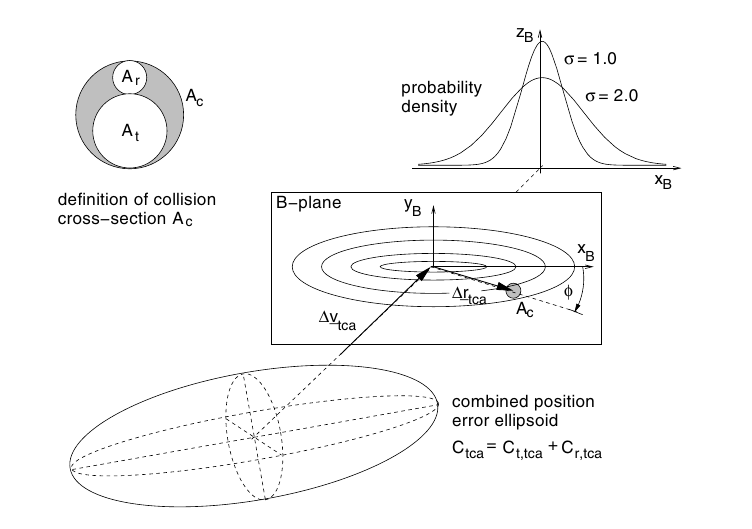
\includegraphics[width=0.5\textwidth]{imagenes/akellabplane}
 \caption{ B-plane (Adaptado de ....)}
 \label{fig:bplane}
\end{figure}

Bien, consideremos ahora una posici\'on relativa de acercamiento $\Delta r_{B}$ ya proyectada en el B-plane. La integral de volumen de la probabilidad de colisi\'on de la Eq. \ref{eq:poc3d} se reduce a una integral de superficie sobre la secci\'on circular de colisi\'on $R_{c}$, proyectada en el B-plane y centrada a la distancia relativa predicha en el instante de m\'aximo acercamiento, $\Delta r_{tca}$

\begin{equation}
P_{c} = \frac{1}{2 \pi \sqrt(det(C_{B}))} \int_{-R_{c}}^{+R_{c}} \int_{-\sqrt(R^{2}_{c}-x^{2}_{B})}^{+\sqrt(R^{2}_{c}-x^{2}_{B})} exp [- A_{B}] dy_{B} dx_{B}
\end{equation}

\begin{equation}
A_{B}=\frac{1}{2}\Delta r^{T}_{B} C^{-1}_{B} \Delta r_{B}
\end{equation}

\section*{Resumen}
A partir de la recepci\'on de informaci\'on respecto de una posible colisi\'on, ya sea mediante un mensaje estandarizado CDM o mediante otros medios, se inicia un an\'alisis de la situaci\'on.\\
A tal fin:\\
\begin{itemize}
 \item Se identifican los objetos involucrados, y se extra su identificador en NORAD y el TCA.
 \item Se solicitan los TLEs de los \'ultimos 15 d\'ias, m\'as pr\'oximos a la fecha del encuentro para el desecho y para la misi\'on operativa en caso de no contar con datos m\'as precisos. Si para la misi\'on operativa se contara con productos orbitales propios se utilizar\'an los errores calculados asociados a los mismos.
 \item Se calcula la matriz de covarianza con el m\'etodo de Osweiler para el desecho (y para la misi\'on si los datos orbitales de la misma no se conocieran).
 \item Se propagan ambas matrices hasta el TCA utilizando los datos estad\'isticos de las tablas generadas, seg\'un la cantidad de d\'ias que se necesite propagar.
 \item Se re\'une toda la informaci\'on y se calcula la probabilidad de colisi\'on.
\end{itemize}

\begin{figure}[!h]
 \centering
 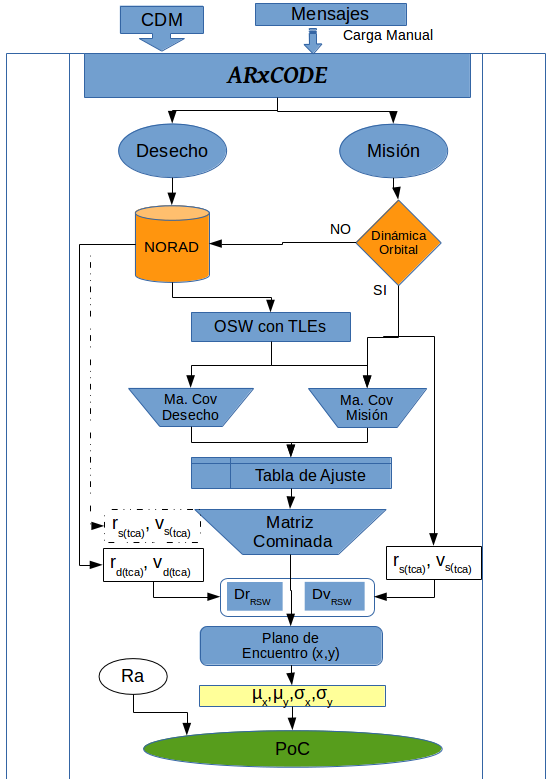
\includegraphics[width=0.7\textwidth]{imagenes/flujomain}
 \caption{Flujo Principal de la construcci\'on te\'orica}
\end{figure}


% \subsection{Tratamiento sobre Datos de Misi\'on}
% En esta etapa repetimos el m\'etodo que propone Osweiler considerando los datos de misi\'on generados por el CODS
% como posici\'on verdadera.\\
% La aplicaci\'on del m\'etodo implica:
% \begin{itemize}
%  \item Identificar el \'ultimo TLE del set: {\it{TLE primario.}}
%  \item Extraer la \'epoca del TLE primario.
%  \item Localizar el archivo CODS que contenga las efem\'erides que encierren la \'epoca del TLE primario.
%  \item Interpolar las efem\'erides de CODS para generar una efem\'eride interpolada a la \'epoca del TLE primario.
%  \item Propagar cada uno de los TLEs del set, hasta la \'epoca del TLE primario.
%  \item Comparar los resultados de las propagaciones con los valores de la efem\'erides interpolada.
% \end{itemize}
% 
% \begin{figure}[!h]
%  \centering
%  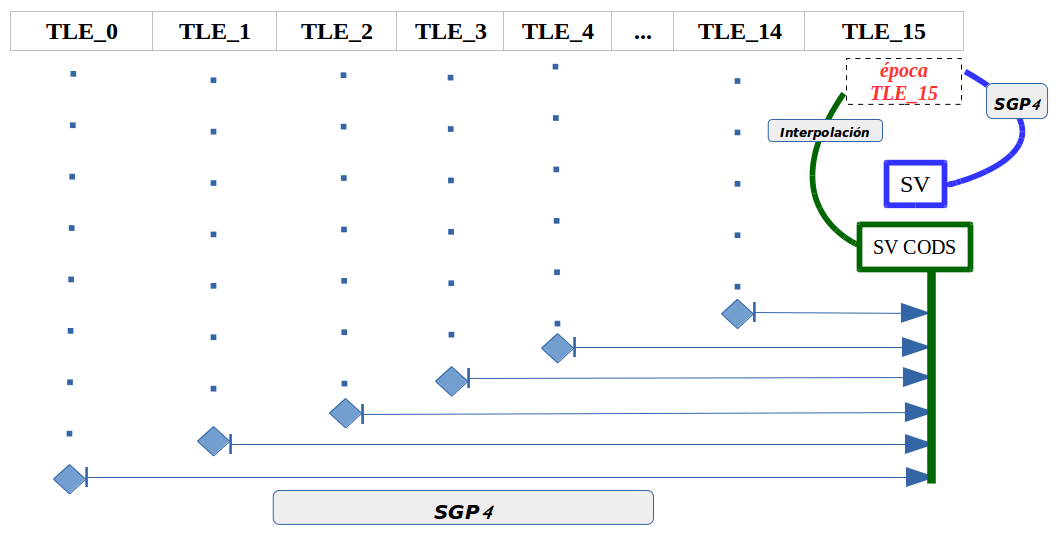
\includegraphics[width=0.7\textwidth]{imagenes/Osweiler_sobre_Cods.png}
%  \caption{M\'etodo de Osweiler sobre datos CODS}
% \end{figure}


